\subsection{2-Wormhole}

%TODO Double check \theta, \phi, y/x, x/y

Consider the quotient space of $\mathbb{H}^2$ generated by quotienting out by a loxodromic transformation. We can set the half-plane model $\mathbb{H}^2 = \{(x,y):y>0\}$ so that the axis of the loxodromic transformation is the $x=0$ geodesic. The loxodromic transformation thus becomes $(x,y) \mapsto e^k(x,y)$ where $k$ is the hyperbolic distance translated along the axis.

%The resulting space is a $(1,1)$-surface of revolution. In particular, the subgroup of the isomorphism group made up by the loxodromic transformations in that direction by arbitrary distances is $S^1$.

The above quotient identifies the semicircles in figure \ref{fig:coordinatecurves}. The resulting quotient space is homeomorphic to $S^1 \times \mathbb{R}$.

%This quotient space can be mapped to $S^1 \times \mathbb{R}$ by $\phi:\mathbb{H}^2 \to S^1 \times \mathbb{R}$ given by $$\phi(x,y) = \left(\frac{2\pi}{k}\log\sqrt{x^2+y^2},\frac{x}{y}\right).$$ %This is necessary to allow it to be generalized to an $(n,1)$-surface of revolution.

The family of functions $(x,y) \mapsto e^d(x,y)$ maps to automorphisms on this quotient space. Since these automorphisms fix radial lines, it would be convenient for one coordinate in the quotient space to be along radial lines. In addition, semicircles about the origin correspond to geodesics, and are fixed by automorphisms in the family $(x,y) \mapsto e^d\left(\frac{1}{x},\frac{1}{y}\right)$, which are the point inversions about the origin. It will be convenient for the other coordinate in the quotient space to move along these geodesics.

\begin{figure}[h]
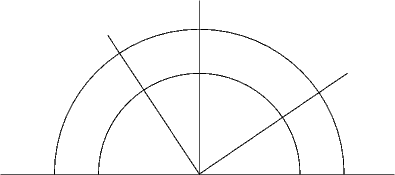
\includegraphics[scale=0.5]{../images/RadialLines.png}
\caption{Coordinate Curves for 2-Wormhole}
\label{fig:coordinatecurves}
\end{figure}

The obvious coordinate system to allow these coordinate curves is polar coordinates: $(r,\phi) = \left(\sqrt{x^2+y^2},\arctan\frac{y}{x}\right)$. This will be a useful starting point, but it can be further improved.

Under polar coordinates, multiplying $x$ and $y$ by $e^k$ corresponds to multiplying $r$ by $e^k$. This increases $\log r$ by $k$, and thus increases $\frac{2\pi}{k}\log r$ by $2\pi$. If we use $\frac{2\pi}{k}\log r = \frac{2\pi}{k}\log\sqrt{x^2+y^2} = \frac{\pi}{k}\log(x^2+y^2)$ as the first coordinate, then the quotient on $\mathbb{H}^2$ is equivalent to quotienting the coordinate by addition of $2\pi$. Since taking that quotient on $\mathbb{R}$ results in $S^1$, we can let $\theta = \frac{\pi}{k}\log(x^2+y^2)$ be one of the coordinates.

I have found that rather than using $\theta$ as a coordinate in $\mathbb{R}/[2\pi]$, it's simpler to use $\theta k$ as a coordinate in $\mathbb{R}/[2\pi k]$. Since $\theta k = \pi\log(x^2+y^2)$, the computations will be independent of $k$, and I just change $k$ by changing the quotient on $\mathbb{R}$.

The choice for the other coordinate is less significant. Any monotonic function of $\phi$ will work. We will use $t = \cot\phi = \frac{x}{y}$, since it's easy to calculate. I chose $\frac{x}{y}$ rather than $\frac{y}{x}$ because $y > 0$, so $\frac{x}{y}$ is always defined.

This gives the coordinate system $$(t,\theta k) = \left(\frac{x}{y},\pi\log(x^2+y^2)\right)$$ for the $2$-Wormhole.

%Vectors must still be rotated.

In addition to mapping the points between the half-plane coordinates and the $2$-Wormhole coordinates, we have to be able to convert vectors between the two. The vectors used in the half plane model are set so that $(0,1)$ points to the point at $(0,\infty)$ and $(1,0)$ is $90^\circ$ clockwise of this.

For the $2$-Wormhole, at $(x,y)$ in half-plane coordinates, the $2$-wormhole vector $(0,1)$ should point in the direction of $(1+\epsilon)(x,y)$, and $(1,0)$ should point $90^\circ$ counter-clockwise of this. We'll now compute the matrices to transform between these vector coordinates.

Suppose you're at point $(x,y)$ in $\mathbb{H}^2$. Let $\phi = \cot^{-1}\frac{x}{y} = \tan^{-1}\frac{y}{x}$. The vector $(0,1)$ in wormhole coordinates should correspond to the direction of $(x,y)$ in $\mathbb{H}^2$ coordinates. This is $(\cos\phi,\sin\phi)$.

The vector $(1,0)$ in wormhole coordinates should correspond to the direction $90^\circ$ counter-clockwise. This comes out to $\mat{0}{-1}{1}{0}\vect{\cos\phi}{\sin\phi} = \vect{-\sin\phi}{\cos\phi}$.

Using this, the matrix to convert from wormhole coordinates to $\mathbb{H}^2$ coordinates should be $\mat{-\sin\phi}{\cos\phi}{\cos\phi}{\sin\phi}$. This matrix is its own inverse, so it can be used to convert either way.

%Add stuff for finding the rotation of a point that has moved.

The final problem is finding the rotation of a point that has moved from $p$ to $q$. Since this is an orientation-reversing map, the rotation must be inverted.

The angle of counter-clockwise rotation $\psi'$ on the wormhole map is $-\psi-(\phi_1-\phi_0)$ where $\psi$ is the angle of counter-clockwise rotation from the parallel transport along the geodesic between $p$ and $q$ on the upper half-plane, $\phi_0$ is $\cot^{-1}\frac{x_0}{y_0}$ where $(x_0,y_0)$ are the half-plane coordinates of $p$, and $\phi_1$ is $\cot^{-1}\frac{x_1}{y_1}$ where $(x_1,y_1)$ are the half-plane coordinates of $q$.

This gives the rotation matrix $\mat{\cos\psi'}{-\sin\psi'}{\sin\psi'}{\cos\psi'}$.

%It might be a good idea to add where $-\psi-(\phi_1-\phi_0)$ came from.